%===================================== CHAP 1 =================================

\chapter{Introduction}

\section{The course}

The goal of the course IT2901 was to give students experience in working on a project with a customer. The students would work in groups to develop a product related to information technology. This included all parts of the software development process, up to, albeit excluding the maintenance/evolution phase.

\section{The customer and project description}

Our group's customer was Forsvarets Forskningsinstitutt (hereby denoted as FFI). FFI is a governmental organization responsible for research and development for the Norwegian Armed Forces. In addition, the organization is involved in the long term plannning of the armed forces, as well as participating in other non-military research projects.

FFI was in need of an application aimed at translating between varied publish/subscribe communication protocols used internally in the Norwegian Armed Forces and the NATO standard protocol for this type of communication, which is the WSNotification protocol.

FFI did at the time not have such an application. They do however own an implementation of the WSNotification protocol, created by a previous IT2901 group in 2014. The group's motivation with respect to this project was mainly the possibility to contribute to providing efficient combat and/or other situational communications between vehicles, stations, personell, unmanned aerial vehicles (UAV) and international NATO forces. This project could yield an important application that will allow quicker adaptation of new devices and tools by the Norwegian Armed Fores, that use other protocols than the NATO standard.

The task of this project was to implement a multi-protocol publish/subscribe brokering solution. Although there exists severeal different publish/subscribe frameworks and protocols, the goal was to make one solution which covered, and was able to translate between several of them. The primary functionality however, was for the solution to support WS-Notification, AMQP and MQTT. The customer wished that the application should be able to translate to and from all the implemented protocols supported, regardless of their type. The application also had to include a graphical interface for administration.

Finally, there were no clear security requirements defined, as the customer assured the group that security lay in the internet layer (e.g IPSec) or link layer (e.g L2TP).

\section{Development methodology}

The choice of development methodology was a result of the project specification, and the group's prior knowledge and experience. The application had some core functionality which had to be implemented.

Other than that, the size of the project was somewhat defined by how much we were able to develop, given the time we had available. This, along with the customer not defining any clear security requirements, called for an iterative and incremental development methodology. Due to this, the team chose Scrum as a basis development methodology. All of the members had prior knowledge and experience with this development methodology.

Scrum specific events and tools were used, as well as more general software development strategies. The customer was located at Kjeller, due to this, customer meetings was mainly held over Skype group meetings.

\section{Project Organization}

The group consisted of six students, studying computer science at NTNU and started fall 2012. Although the background of the group is similar, group roles were distributed in order to complement the individual skills of each team member.

After discussing with the customer, the team decided to have iterations lasting two weeks, starting Monday 26 of January. The two weeks gives the group room to plan according to mandatory work in other courses. The customer also recommended and preferred having biweekly meetings. Furthermore, a distribution of roles have been made, as defined below. 

\subsection{Product owner}

The product owner was Frank T. Johnsen from FFI, which is the main voice of the customer. Johnsen was responsible for communication with the development team, and also had the responsibility for providing the group feedback about the process and product. In this case, Johnsen was not participating in any of the development.

\subsection{Scrum Master}

Trond Walleraunet was given the role of scrum master. This is due to him having some prior acquaintance with the customer, as well as prior experience in the role. A scrum master has the main responsibility for monitoring progress and deliverables, as well as being the main communication link between the team and the customer.

\subsection{Development team}

The other five members of the group constituted  the development team. The team and the scrum master is responsible for developing the product, as well as completing the other deliverables in time. In order to distribute some responsibility away from the Scrum master, the group has assigned members to these areas of the project

\subsubsection{Report and documentation}

<Insert navn> was responsible for distributing work regarding written deliverables and documentation writing.

\subsubsection{Architecture}

Decisions regarding the architecture was mainly considered in the early to middle phases of the project. It was however, important to ensure that the foundation of the system is developed in a well formed fashion.

\subsubsection{Lead developer}

The lead developers role was keeping control of the progress of the development part of the project. The role was given to <Insert navn> due to his experience and knowledge of the development environment. Time management and control of written code were the main tasks of the lead developer.

\subsubsection{Testing and configuration management}

The role was given to <Insert navn>, who had the responsibility of writing tests. He was also responsible for research and execution of test methodology.

\subsubsection{Design and user experience}

<Insert navn> was mainly responsible for the front end part of the project. 
\section{Time management}

This is the current time table, including dates indicating major deliverables.

\begin{center}
  \begin{figure}
    \makebox[\textwidth]{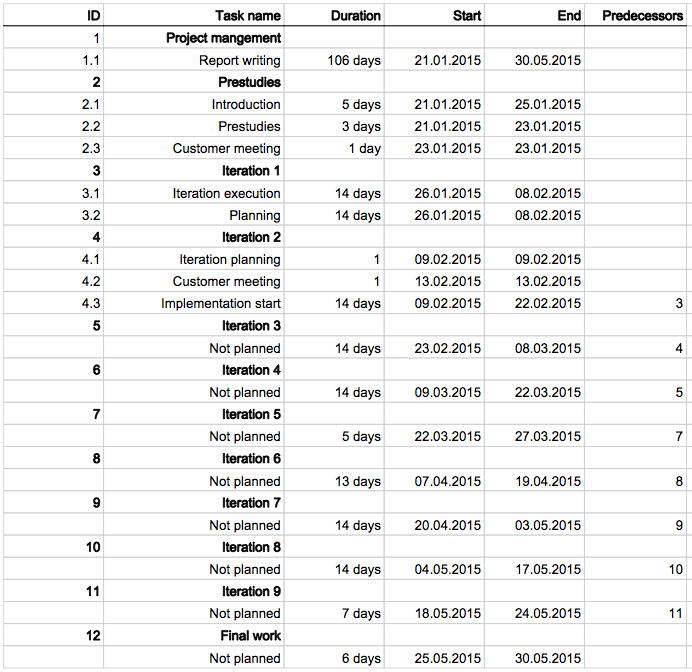
\includegraphics[width=\textwidth]{fig/Gantt.png}}
    \caption{Gantt diagram}
    \label{fig:gantt}
  \end{figure}
\end{center}

\begin{center}
  \begin{figure}
    \makebox[\textwidth]{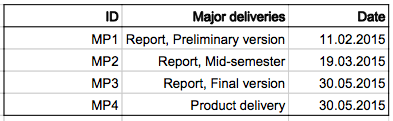
\includegraphics[width=\textwidth]{fig/Deliverables.png}}
    \caption{Major deliverables}
    \label{fig:deliverables}
  \end{figure}
\end{center}

\begin{center}
  \begin{figure}
    \makebox[\textwidth]{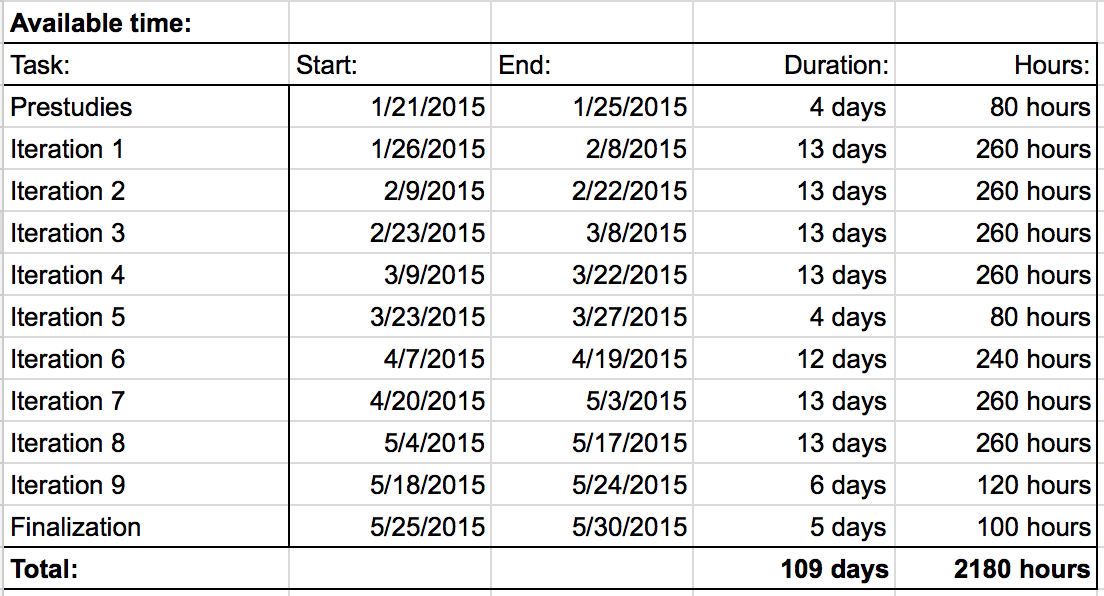
\includegraphics[width=\textwidth]{fig/available_time.png}}
    \caption{Available time}
    \label{fig:available_time}
  \end{figure}
\end{center}

\cleardoublepage